% !TEX root = ../main.tex
% !TEX program = XeLaTeX
% !TEX encoding = UTF-8 Unicode

\date{2018년 3월 7일}

\begin{frontmatter}
\title{축치어}
\author{김민규}
\address{서울대학교}
\begin{abstract}
Dunn, Michael. (1999). A Grammar of Chukchi. PhD dissertation, Australian National University, 1--60.
\end{abstract}
\end{frontmatter}

%%%%%

\section*{발제 범위 분배}
\begin{table}[h]
\begin{center}
\def\arraystretch{1.5}
\begin{tabular}{>{\sffamily}ccccl}
\hline
	&\itshape 발제자	&\itshape 발제 범위		
	&\itshape 페이지	&\itshape 내용\\
\hline
1	&김민규	&Ch. 1--3	&pp. 1--60		&서론, 방언, 음운론 \& 형태음운론\\
2	&		&Ch. 4--6	&pp. 61--118		&품사, 문장, 명사 굴절\\
3	&		&Ch. 7--9	&pp. 119--174	&대명사, 명사 파생, 복합 명사\\
4	&		&Ch. 10--11	&pp. 175--220	&동사 굴절, 결합가\\
5	&		&Ch. 12--13	&pp. 221--252	&동사 포합, 비정형 동사파생 형태\\
6	&		&Ch. 14--15	&pp. 253--290	&동사 파생, 장소적 관계\\
7	&		&Ch. 16--17	&pp. 291--324	&형용사 \& 수사, 계사 \& 보조사\\
8	&		&Ch. 18--19	&pp. 325--360	&부정문, 화용론\\
\hline
\end{tabular}
\end{center}
\label{default}
\end{table}

%%%%%

\section{서론}
\begin{itemize}
\item 본 연구는 축치어의 텔케프(Telqep) 방언의 문법을 기술한다.
\item 축치어는 시베리아의 동쪽 끝 축치 자치주(추콧카)에 주로 거주하는 축치인의 언어이다. 
\item 에스놀로그의 2010년 조사에 의하면 15900명의 축치인 중 5100명이 축치어를 할 줄 안다. 
\item 축치어 사용은 줄어드는 추세이며 ``심각하게 위기에 처한 언어''로 유네스코 레드북에 등재되어 있다.
\item 지금까지의 축치어 문헌은 주로 인공적인 문어체인 ``표준 축치어''를 다뤘으며 방언 차이를 간과해 왔으나, 본 연구는 텔케프 방언의 구어체를 다루며 단일언어 구사자들의 자발적 발화에 바탕을 둔 첫 연구이다.
\end{itemize}

\subsection{축치 문화}
\begin{itemize}
\item 축치인의 생활방식은 유럽인과의 접촉 이후에도 20세기 중반까지 큰 변화가 없었다. 
\item 축치인은 원래 순록 유목으로 먹고 살았고 여기에 더해 사냥, 낚시, 식물 채집을 했다. 
\item 인구 증가 때문에 일부 축치인은 바닷가에 정착해 살며 바다에서 식량을 구하게 되었다. 축치 사회는 크게 툰드라 유목민과 해안 정착민으로 구분되었다. 
\begin{itemize}
\item 해안 정착민은 툰드라 유목민을 Cawcəwat (sg. Cawcəw, 순록치는 사람이라는 뜻) 이라 불렀다. 
\item 이를 차용해 이웃한 퉁구스계 민족들은 축치인을 čävča라 불렀다. 
\begin{itemize}
\item 축치(\textsc{m. sg.} чукча \textit{chukcha})라는 러시아어 이름은 여기서 나온 것으로 보인다.
\end{itemize}
\item 현대에 순록 치는 축치인들은 소련 집단농장의 유산인 농장에서 일하고 있다. 
\item 몇몇 축치인은 순록떼 근처 캠프에서 살지만 대부분의 축치인은 아파트 단지에서 산다.
\end{itemize}
\end{itemize}

\subsubsection{성 역할}
\begin{itemize}
\item 전통적으로 남녀의 역할은 구분되어 있다.
\begin{itemize}
\item 남성은 사냥을 하고 목축을 주로 맡았다. 
\item 여성은 식물을 채집하고 순록 가죽을 다루며 자식을 양육했다.
\end{itemize}
\item 남녀의 축치어 발음은 상당히 다르지만 이상하게도 여성의 축치어에 대한 문헌은 거의 없다.
\item 오늘날에도 모든 축치 여성은 여성 방언으로 말한다.
\item 본 연구는 여성 방언에 큰 관심을 기울였다.
\end{itemize}

\subsubsection{언어와 마술}
\begin{itemize}
\item 샤머니즘과 전통 종교는 소련의 탄압을 받았지만 아직까지 남아 있다.
\item 저자는 현업 샤먼을 만나보진 못했고 죽은 샤먼의 자녀와 은퇴한 샤먼은 만나보았다.
\item 샤먼은 자신과 반대 성별의 옷차림을 하고 반대 성별의 방언을 사용했으며 다른 면에서도 반대 성별처럼 행동했다.
\end{itemize}

이하 1.1.3. -- 1.1.6. \omission

\subsection{언어적 상황}
\begin{itemize}
\item 축치어와 친척인 언어는 매우 적다. 알루토르어(Alutor), 코랴크어(Koryak), 케레크어(Kerek)는 모두 축치와 가까운 친척이다. 이들을 묶어 코랴크·축치어파((Koryako-)Chukotian)라 부른다. 
\item Comrie (1981:240)는 이들이 한 언어의 방언으로 봐도 될 만큼 비슷하다고 말한다.
\item 여기에 이텔멘어(Itelmen) 또는 캄차달어(Kamchadal)를 더하여 축치·캄차카어족(Chukotko-Kamchatkan)이라 부르는데, 증거가 불충분하여 논란의 여지가 있다.
\end{itemize}

\subsubsection{언어 접촉}
17세기 기준으로 축치어와 인접해 있던 언어들은 다음과 같다.
\begin{itemize} 
\item 코랴크어 방언들이 있었다. 알루토르어와 케레크어 사용자들은 수가 훨씬 적었고 축치인들에게 동화되어 현재는 화자가 남아 있지 않거나 극소수만 남아 있다. 
\item 튀르크어족의 야쿠트어(Yakut)와 퉁구스어족의 어웡어(Even)가 있었다. 
\item 에스키모 언어들이 있었다. 에스키모들과 축치인들은 많은 영향을 주고받았다. 에스키모 언어들은 축치어 어휘, 특히 바다와 관련된 영역에 영향을 끼쳤다. (축치어 puwreq < Eskimo puwreq ‘beluga whale’ 등)
\item 축치인은 17세기부터 러시아인과 접촉했다. 미국인과 캐나다인도 19세기 동안 추콧카에서 활동하였다. 축치어는 러시아어와 영어로부터 차용어를 받아들였다.
\end{itemize}

\subsection{연구 조건}
\omission
\subsection{데이터}
\omission
\subsection{선행 연구 조사}
\omission

\section{방언 변이}
\subsection{서론}
\begin{itemize}
\item 축치어의 지리적 변이는 크지 않으며 주로 어휘부에 나타난다. 
\item 동사 일치 체계 및 다른 문법에서도 몇몇 차이점이 있다. 
\item 축치어파 언어들 사이의 차이도 크지 않아, 문화적/역사적 요인이 아니면 하나의 언어로 불릴 수 있을 정도.
\item Skorik 가 기술한 ‘표준 축치어(Standard Chukchi)’ 또는 ‘문어체 축치어(Literary Chukchi)’는 여타 방언과는 사뭇 다르다. 
\begin{itemize}
\item 지금까지 축치어에 관한 이론적 논의는 자료 접근성 문제 때문에 주로 이 인공적인 방언을 데이터의 출처로 삼았는데 저자에 의하면 여기에는 문제가 많다.
\end{itemize}
\end{itemize}

\subsection{언어학적 비교}
축치어파 언어들의 분화는 비교적 최근에 일어난 것으로 보인다. 
\subsection{성별 방언}
\begin{itemize}
\item 남성의 축치어와 구별되는 여성의 축치어가 있다는 사실은 잘 알려져 있었지만, 여성의 축치어를 다룬 문헌은 거의 없었다. 
\item 이전의 연구에서는 둘의 차이가 단순히 한 소리를 다른 소리로 발음하는 정도의 차이라고 주장했으나, 본 연구는 둘의 차이가 그보다 더 복잡한 현상임을 밝힌다. 
\item 사실 여성 방언형과 남성 방언형의 대응 관계는 공시적으로 예측 불가능하며, 축치어파 언어들에 대한 방언학적 지식이 있어야 완전히 설명할 수 있다.
\item 성별 방언은 비록 드물지만 세계 각지에서 관찰되는 현상이다. (Island Carib (Hoff 1994), Pirahã (Everett 1986:317), Yana (Sapir 1963) 등)
\item 남성의 축치어와 여성의 축치어는 실제로 서로 다른 지리적 방언들과 연관되어 있음을 보일 수 있다. 
\item 특기할 만한 점은 축치어를 제외한 어느 축치어파 언어도 성별 방언이 존재하지 않는다는 사실이다. 따라서 성별 방언은 축치어가 다른 언어들로부터 갈라져 나온 뒤에 생겨난 현상임을 짐작할 수 있다.
\end{itemize}

\subsubsection{사회언어학적 지위}
\begin{itemize}
\item 어느 성별 방언을 사용하는가는 화자의 성별에 달려 있다. 반대 성별의 방언을 말하는 것이 금지되어 있지는 않다. 다른 사람을 인용할 때, 인용되는 사람의 성별 방언형으로 말하기도 한다. 
\item 성별 방언형의 대응 관계는 예측 불가능하므로, 다른 방언형을 알려면 암기하는 수밖에 없다. 
\item 전통 사회에서 샤먼의 힘은 성별의 부분적인 또는 완전한 전환과 연결되곤 했다. 언어는 성별의 두드러진 지표이므로 샤먼과 샤먼의 대상들은 반대 성별의 방언으로 말하는 경우가 자주 있었다. 축치인 남녀는 반대 성별의 방언도 잘 알고 있다.
\begin{itemize}
\item 소련 치하에서 축치인의 샤머니즘은 폭력적으로 탄압되었으며 여성 축치어의 사용은 장려되지 않았다. 축치어 표준화 작업은 순전히 남성 방언을 기반으로 했다. 1990년대에 들어서, 교육받은 여성들은 여성 축치어 사용을 다소 부끄러워하는 듯하지만 여전히 잘 사용하고 있다. 축치어 라디오와 텔레비전은 모두 남성 방언으로만 방송된다. 여성 아나운서들도 남성 방언으로 방송한다. 여성이 남성 방언을 사용하는 것은 모르는 사람들 앞에서의 공개 연설에서뿐이다. 남성들도 여성 방언을 할 줄 알지만 여성 방언으로 말하도록 요구받는 상황은 극히 드물다.
\end{itemize}
\end{itemize}

\subsubsection{r $\sim$ c 교체 현상}
\begin{itemize}
\item 공시적으로 예측 불가능한 특정 환경에서 남성 방언의 r은 여성 방언의 c에 대응한다. 
\item 이외의 환경에서는 남성 방언의 r과 c가 그대로 여성 방언의 r과 c에 대응한다.
\begin{center}
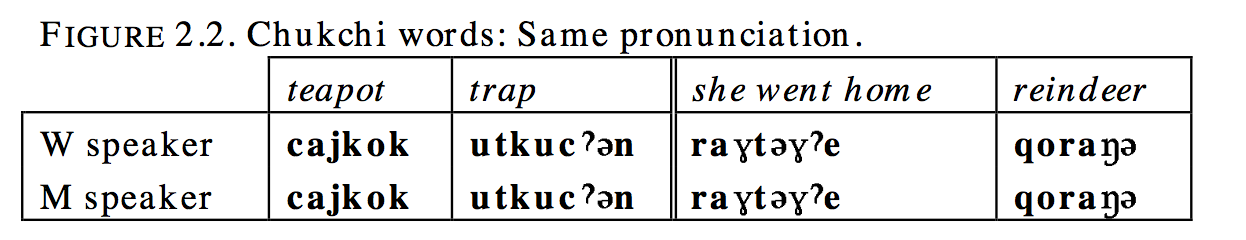
\includegraphics[width=.8\linewidth]{Chukchi/src/Chukchi-rc}
\end{center}
\item Muravyova (1979)는 축치어파 언어들의 음운 대응을 설명하면서 코랴크·축치조어에 자음 *d가 존재했다고 주장하였다. 저자가 여성 축치어를 연구한 결과, 축치어 남녀 방언의 r $\sim$ c 교체는 Muravyova의 *d에 대응함이 밝혀졌다. *d의 변화를 보면 여성 축치어는 뜻밖에도 남성 축치어--차브추프코랴크어 방언군보다는 알루토르어--팔라나코랴크어 방언군에 더 가까워 보인다. 즉 축치어 성별 방언은 어떤 코랴크·축치어파의 지리적 방언이 한쪽 성별의 축치어 화자들에게 기층 영향을 미친 결과라는 가설을 세울 수 있다. 두 성별 중 여성의 축치어가 영향을 받았을 가능성이 더 높아 보인다. 축치 여성은 결혼 뒤에 남편의 마을로 이주하기 때문이다. *d의 등언어선 경계를 넘어 이주한 여성들이, 자기 방언의 간섭으로 인하여 축치어를 말할 때 발음 실수를 범했을지도 모른다. 축치 사회에서 남녀의 역할은 뚜렷이 구분되었으므로, 일부 여성의 특징적 발음 실수가 사회적으로 여성성의 표지가 되는 상황을 상상해봄직하다.
\end{itemize}

\subsection{축치어 내 지리적 변이}
\omission
\subsection{표준 축치어}
\omission

\section{음운론 \& 형태음운론}
\subsection{서론}
\begin{itemize}
\item 축치어 텔케프 방언의 음운론과 형태론을 기술하는 장이다.
\begin{itemize}
\item 음운론적, 형태론적 교체 현상을 설명하고 전사의 원칙들을 설명한다.
\item 음운론 기술은 이론 중립적일 수 없지만 최대한 논란의 여지가 없게끔 노력했다.
\item 전통적인 음운, 음운론적 자질, 운율론적 음운/자립분절음운 등의 개념을 포함한다. 
\end{itemize}
\item 음운론 개괄
\begin{itemize}
\item 자음 13개 /p t k q m n ŋ ɬ s w ɾ j ɣ/
\item 모음 조화와 성문음화(때때로 14번째 자음 취급)가 존재한다.
\item 모음 기저형 3개 /*i *e *u/ 실현형 /i e a o u/ (+삽입모음 /ə/)
\item 최근 모음 장단에 의한 구별이 생겨나고 있다. (자매 언어에는 존재하지 않음)
\item 몇 가지 동화와 이화 현상이 형태론/단어 경계에서 일어난다.
\item 남성과 여성의 음운론적 체계가 상이하다.
\end{itemize}
\item 3 종류의 전사 체계 (키릴 문자, 라틴 문자, IPA 기반)가 존재한다.
\end{itemize}

\subsection{단어 형성}
\begin{itemize}
\item 모음조화로 음운론적 단어 경계를 조사하기 쉽다.
\item 음운론적 단어는 대부분의 경우 문법적 단어와 일치하지만 몇 가지 예외가 있다.
\begin{itemize}
\item 강조 접어(emphatic clitic) \textbf{=ˀm} (4.8.9 참조)
\item 여러 음운론적 단어가 모여 하나의 문법적 단어처럼 행동하는 경우가 존재한다. (4.1 참조)
\end{itemize}
\item 축치어의 음성적 실현은 일련의 형태소에 규칙을 적용하여 생성할 수 있다.
\item 분절적 음운 외에도 운율론적 음운과 성절화가 존재한다.
\end{itemize}

\subsubsection{CV 뼈대}
\begin{center}
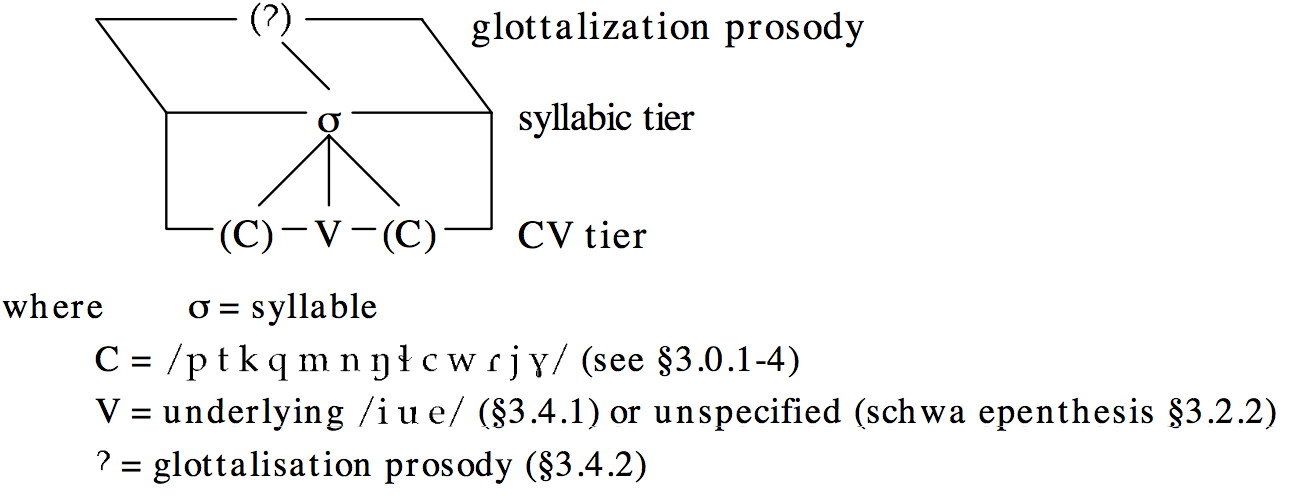
\includegraphics[width=.8\linewidth]{Chukchi/src/Chukchi-CVskeleton}
\end{center}
\begin{itemize}
\item 축치어 단어는 1개 이상의 음절로 구성되며 각 음절은 σ = (C)V(C) 구조를 가진다.
\item 모음은 기저형에서 존재하지 않을 수 있다. 이 때에는 삽입모음 /ə/ 으로 실현된다.
\item 각 음절은 성문음화가 일어날 수도, 일어나지 않을 수도 있다.
\item 단어 내의 모든 음절은 모음 조화된다. 
\end{itemize}
\begin{center}
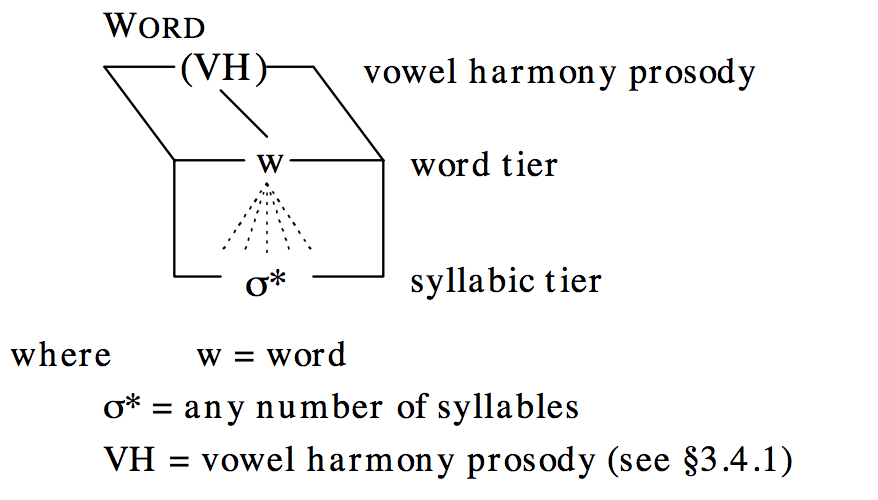
\includegraphics[width=.6\linewidth]{Chukchi/src/Chukchi-VH}
\end{center}

\subsubsection{성절화 및 모음삽입}
\begin{itemize}
\item \textbf{결합 법칙}
\begin{itemize}
\item 주어진 CV 뼈대를 이용해 오른쪽에서부터 왼쪽으로 결합을 진행한다. 각 음절은 최대한 많은 구조상 원소들과 결합한다. 어두 모음이 존재할 때를 제외하고는 항상 두음이 채워진다.
\end{itemize}
\item 대부분의 /ə/는 삽입모음으로 해석할 수 있다. 그러나 몇 가지 예외가 존재한다. 인칭-수 접미사 -tkə, -tək 가 최소대립쌍을 이룬다.
\begin{itemize}
\item /ə/가 모음 음소일 수 있다.
\item 기저형의 성절화 방식이 지정될 수 있다. 
\end{itemize}
\end{itemize}

\subsubsection{모음 삭제}
\begin{itemize}
\item -V\textsubscript{1}V\textsubscript{2}- $\rightarrow$ -V\textsubscript{2}-; 축치어에는 이중모음이 존재하지 않는다.
\end{itemize}

\subsubsection{모음-접근음 동화 (장모음)}
\begin{itemize}
\item -V\textsubscript{1}C\textsubscript{approx}V\textsubscript{2}- $\rightarrow$ -V\textsubscript{2}V\textsubscript{2}- (e.g. /ˀoɾacek/ $\sim$ /ˀaacek/ `youth, lad’)
\item 19세기 후반 -- 20세기 초반의 변화이며 남성 방언에서 시작되었다.
\item 몇몇 형태들은 변화된 형태로 굳어졌으며 몇몇은 변화하지 않았고, 아주 조금은 두 가지 형태가 모두 사용된다.s
\end{itemize}


\subsection{자음 음소}
\begin{center}
\begin{tabular}{|l|ccccc|}\hline
	&bilabial	&alveloar	&palatal	&vlear	&uvular\\\hline
stops	&p	&t	&	&k	&q\\
nasals	&m	&n	&	&ŋ	&\\
approximants	&w	&ɾ	&j	&ɣ	&\\
frivatives	&	&s/c	&	&	&\\
	&	&ɬ	&	&	&\\
\hline
\end{tabular}
\end{center}

\NB\quad /c/는 /ts/를, /ɣ/는 /ɰ/를 나타낸다.

\subsubsection{파열음}
\begin{itemize}
\item 파열음 /p, t, k, q/은 무성 무기음으로 실현된다.
\item /p/ $\rightarrow$ [m] / \_C[+\textsc{nasal}]; [p] elsewhere
\item /t/ $\rightarrow$ [n] / \_C[+\textsc{nasal}]; [t] elsewhere
\item /k/ $\rightarrow$ [q] / \_q; [ɣ] / \_C[-\textsc{back}] (lenition); [k] elsewhere
\item /q/ $\rightarrow$ [\textsc{glot}] / \_C; [q] elsewhere
\end{itemize}

\subsubsection{마찰음 및 파찰음}
\begin{itemize}
\item /s/는 남성 방언에만 나타난다. 텔케프 방언에서는 [s] $\sim$ [tʃ] 자유변이로 나타난다. (변이음 아님)
\item /c/는 여성 방언에만 나타난다. 다음과 같은 분포를 가지고 있다.
\item /c/ $\rightarrow$ [t] / \_\#; [s] / \_q; [c] elsewhere
\item 표준 축치어는 남성 방언을 기반으로 하고 있지만 /s/를 /q/앞에서만 ⟨с⟩로, 그 외에는 ⟨ч⟩로 적고 있다. 여성 방언의 영향으로 보인다.
\item /ɬ/ $\rightarrow$ [ɬ] $\sim$ [t] / \_ɬ / \_q; [c] elsewhere
\item 설측 마찰음은 /c/ 또는 /s/와 자연 부류를 이룬다.
\end{itemize}

\subsubsection{비음}
\begin{itemize}
\item /m/ $\rightarrow$ [m]
\item /n/ $\rightarrow$ [n]
\item /ŋ/ $\rightarrow$ [α \textsc{place}] / \_C[-\textsc{nasal} α \textsc{place}]
\item /ŋ/ $\rightarrow$ [ɣ] / \_\{m, n\}; [n] / ɣ \_; [ŋ] elsewhere
\item 표준 축치어는 남성 방언을 기반으로 하고 있지만 /s/를 /q/앞에서만 $\langle$с$\rangle$로, 그 외에는 $\langle$ч$\rangle$로 적고 있다. 여성 방언의 영향으로 보인다.
\item 이화 규칙 /ŋ/ $\rightarrow$ [n] / ɣ \_ 은 축치어의 유일한 순행 규칙이다.
\item 축치어에만 나타나는 /ŋ/ $\rightarrow$ [ɣ] / \_C[+\textsc{fricative}] \_ 교체 현상도 존재한다. (형태소 경계에서만 발생)
\begin{itemize}
\item e.g. singulative /apaapaɣ-ɬəŋ-ə-n/ `a (single) spider’ /ɬəɬa-ɬɣ-ə-n/ `an eye’
\item 이 교체 현상이 생산적인지는 분명하지 않다.
\end{itemize}
\end{itemize}

\subsubsection{마찰음 및 파찰음}
\begin{itemize}
\item /w/ $\rightarrow$ [w]
\item /ɾ/ $\rightarrow$ [t] / \_C[+\textsc{coronal}] ; [ɾ] elsewhere
\item /j/ $\rightarrow$ [ɣ] / \_C[+\textsc{coronal}] ; [j] elsewhere
\item /ɣ/ $\rightarrow$ [ɣ]
\item -V\textsubscript{1}C\textsubscript{approx}V\textsubscript{2}- $\rightarrow$ -V\textsubscript{2}V\textsubscript{2}-
\item ə $\rightarrow$ i / j; ə $\rightarrow$ u / w
\item Non-coronal non-nasal clustser $\rightarrow$ /kw/ where at least one of them is /w/ or /ɣ/. (e.g. ww $\rightarrow$ kw)
\end{itemize}

\subsubsection{남성과 여성의 /r/ 및 /c/ $\sim$ /s/}
\omission

\subsection{운율론적 음소 (`운소')}
\subsubsection{모음과 모음 조화}
\begin{itemize}
\item 축치어의 모음 실현형은 /i e a o u/ 5개와 삽입모음 /ə/으로 구성된다. 
\item 이들은 모음 조화를 통해 세 개의 기저형 /*i *e *u/으로 묶을 수 있다.
\begin{center}
\begin{tabular}{|l|ccc|}\hline
$-$VH	&i	&e	&u\\
$+$VH	&e	&a	&o\\
\hline
\end{tabular}
\end{center}
\item 두 가지 /e/는 음성적 차이가 없다.
\item 모음 조화 운소는 분절 음소와 독립적으로 존재하며, 한 형태소가 모음 조화 운소를 가지고 있으면 해당 형태소가 포함된 단어의 전체 모음 조화가 그 운소를 통해 결정된다.
\end{itemize}

\subsubsection{성문음화}
\begin{itemize}
\item 성문 파열음은 반드시 모음 앞에서만 나타날 수 있다. 이는 음소로 취급되지 않는다.
\begin{itemize}
\item 분포가 제약되어 있다. 음절의 최대 형태는 CˀVC 이다. 
\item 형태 중첩(reduplication) 시, 자음과 모음만 복사되고 성문 파열음은 무시된다. (e.g. /wˀaɾe-waɾ/ `fork’)
\end{itemize}
\item 그러나, 성문음화 운소는 존재하는데 자음이 없을 경우, 성문 파열음이 두음으로 나타난다. (e.g. /ˀituˀit/ `goose’)
\item 또한, 성문 파열음이 두 모음을 분리하는 자음으로 존재하는 경우도 존재한다. (e.g. /iˀam/ `why?’)
\end{itemize}

\subsection{음운론적 및 형태음운론적 교체 현상}
\begin{itemize}
\item 
\end{itemize}

\subsection{/r-/ $\sim$ /-n-/ 교체}
\subsection{내부 자음 $\sim$ $\varnothing$ 교체}
\subsection{외부 자음 $\sim$ $\varnothing$ 교체}
\subsection{모음 약화}

\subsection{억양}
\begin{itemize}
\item 자음으로 된 두음과 기저 모음을 가진 첫번째 `완전한 음절’에 제 1 강세가 부여되고, 두 음절마다 제 2 강세가 부여된다.
\end{itemize}
\subsection{정서법}
\omission
